% ===========================================================================
%  user/01-getting-started/00-chapter.tex
% ===========================================================================
\chapter{Getting started}\label{cap:getting-started}

\begin{attenzione}{The numbers in the screenshots are made up}
Every image in this guide was taken on an installation with \emph{sample
data}: series generated by a computer, not real prices and not the results
of real strategies. They are there to show where things are. No Sharpe ratio,
return or drawdown on these pages means anything.
\end{attenzione}

\section{What Lyra does}\label{sez:what-it-does}

Three things, in this order:

\begin{enumerate}
  \item \textbf{Build} an investment strategy --- by writing it, by drawing
        it with blocks, or by describing it in words.
  \item \textbf{Test} it on past data, with costs, and see how it would have
        behaved.
  \item \textbf{Run} it on a real account, when it holds up.
\end{enumerate}

\noindent
Strategies can also be combined with one another, and bought and sold
between users on the marketplace of the \voce{Community}. This guide follows
the same order: one chapter per area of the application.

\figuraTikz{user-flow}
  {The areas of the application, in the order you use them. The arrow that
   goes back is the most frequent part of the work.}
  {user-flow}

\section{The menu}\label{sez:menu}

The bar on the left is always there. It widens when you hover over it with
the mouse and shows the names of the items.

\begin{figure}[htbp]
  \centering
  \setlength{\fboxsep}{0pt}\setlength{\fboxrule}{0.5pt}%
  {\color{lyraGrigioChiaro}\fbox{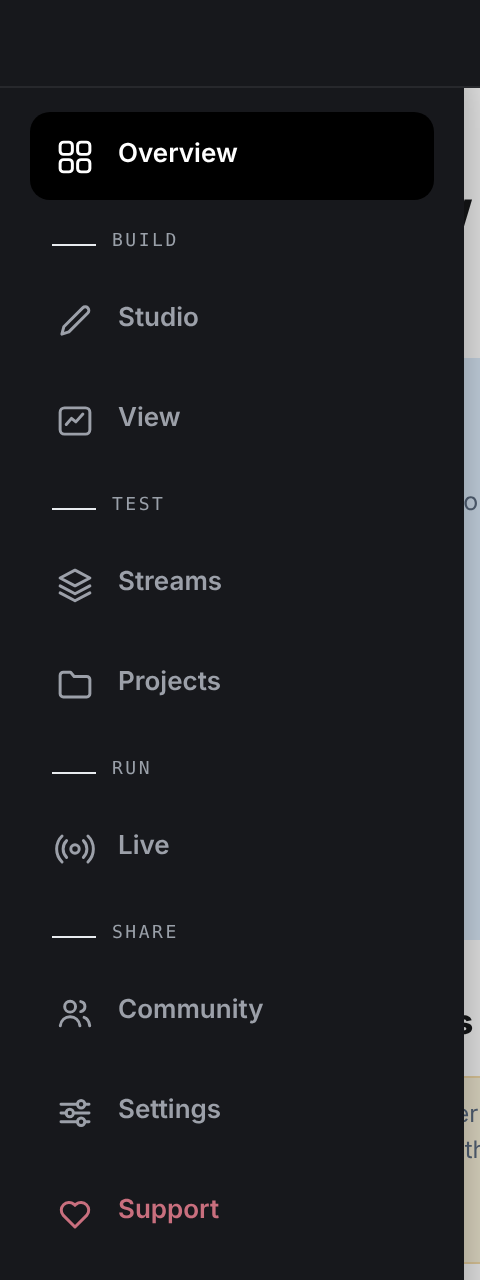
\includegraphics[width = 0.26\linewidth]
    {figure/schermate/menu.png}}}
  \caption{The menu, widened. Below \voce{Overview} the items are in four
           groups --- \voce{Build}, \voce{Test}, \voce{Run}, \voce{Share}.
           \voce{Settings} sits at the bottom.}
  \label{fig:menu}
\end{figure}

\begin{center}
\begin{tabular}{@{}L{26mm}L{18mm}L{90mm}@{}}
\toprule
\textbf{Item} & \textbf{Group} & \textbf{What it is for} \\
\midrule
\rigaTenue
\voce{Overview} & --- & The home screen: how everything is going, on one
  page. \\
\voce{Studio} & Build & Where strategies are built. \\
\rigaTenue
\voce{View} & Build & The charts, with what the strategy did drawn on
  top. \\
\voce{Streams} & Test & The results: one card per strategy. \\
\rigaTenue
\voce{Projects} & Test & Combinations of several strategies. \\
\voce{Live} & Run & The link to a real account. \\
\rigaTenue
\voce{Community} & Share & The strategy marketplace, messages, feedback and
  your own account. \\
\voce{Settings} & --- & Data, parameters, market regimes. \\
\bottomrule
\end{tabular}
\end{center}

\begin{nota}{Top right}
The magnifying glass searches the whole application; the bell shows finished
jobs and messages; the sun switches between light and dark; the last item is
the way into your account.
\end{nota}

\section{Do you need an account?}\label{sez:account-needed}

To build, test and run strategies, \textbf{no}: the application runs on your
own computer and asks for nothing.

An account is needed only for the areas that go through the network: the
\voce{Community} --- marketplace, messages, feedback, profile --- and the
subscription. If you open one of them without being signed in, the
application says so and offers to sign you in.

\section{The order in which you work}\label{sez:order}

\begin{pratica}{From nothing to the first result}
\begin{enumerate}
  \item \percorso{Settings \freccia Data}: download the data. Without data,
        every page is empty --- it is not an error, there is simply nothing
        to show.
  \item \percorso{Streams \freccia Run backtest}: choose a strategy and press
        \pulsante{Run backtest}.
  \item Wait. The job runs in the background and the bell tells you when it
        is done; meanwhile you can use the rest of the application.
  \item \voce{Streams}: the result has appeared as a card.
  \item \voce{Projects}: combine two or more results.
  \item \voce{Live}: connect a broker, when you are ready.
\end{enumerate}
\end{pratica}
